% -- LaTeX rewrite of main.typ, using the OUP template and matching the structure and content --

\documentclass[unnumsec,webpdf,contemporary,large]{oup-authoring-template}
\usepackage{booktabs}

\theoremstyle{thmstyleone}%
\newtheorem{theorem}{Theorem}%
\newtheorem{proposition}[theorem]{Proposition}%
\theoremstyle{thmstyletwo}%
\newtheorem{example}{Example}%
\newtheorem{remark}{Remark}%
\theoremstyle{thmstylethree}%
\newtheorem{definition}{Definition}

\begin{document}

\journaltitle{Journal Title Here}
\DOI{DOI HERE}
\copyrightyear{2022}
\pubyear{2019}
\access{Advance Access Publication Date: Day Month Year}
\appnotes{Paper}

\firstpage{1}

\title[Short Article Title]{Assessing the Reliability of AlphaFold3 Predictions for Protein-Ligand Affinity Prediction via Sfcnn}

\author[1]{Guo Yu \thanks{Student ID: 2022533074}}
\author[1]{Yiming Wu \thanks{Student ID: 2023591024}}
\author[1]{Yiyang Tan \thanks{Student ID: 2023533142}}

\authormark{Guo Yu et al.}

\address[1]{\orgdiv{School of Information Science and Technology}, \orgname{ShanghaiTech University}, \orgaddress{\street{393 Middle Huaxia Road}, \postcode{201210}, \state{Shanghai}, \country{China}}}




\abstract{
This project investigates the reliability of using AlphaFold3 (AF3)-predicted 
structures as an alternative. Sfcnn, a 3D-CNN based protein-ligand affinity prediction model, 
is reproduced using PyTorch, and its performance is validated on the PDBbind v2019 refined set 
for training and the CASF-2016 core set for testing. The AF3-derived protein structures of 
CASF-2016 core set are then evaluated and compared against the groundtruth and Sfcnn scores 
on the core set to assess the viability of AF3 predictions in PLA tasks.
}
\keywords{AlphaFold3, protein-ligand affinity, CNN scoring function, CASF-2016}

\maketitle

\section{Introduction}

\subsection{Sfcnn Background}
Sfcnn is a 3D convolutional neural network based scoring function model proposed in 2022, 
which aims to provide accurate and reliable scores for binding affinities of protein-ligand 
complexes.

\section{Data Methods}

\subsection{Dataset}
The Sfcnn network was trained with protein-ligand complexes from the refined set of the PDBbind database version 2019, 
which contains protein-ligand complexes and their corresponding binding affinities expressed with pKa values. 
The trained network is later tested on the CASF-2016 core set, which has 285 protein-ligand complexes.

Note that the overlaps between train set and test set (266 protein complexes) are excluded, 
leaving 4852 train complexes in total.

\subsection{Augmentation}
To scale up the training set, each protein-ligand complex is rotated randomly for 9 times 
using random rotation matrices. Those 10 complexes should bear the same PLA 
(protein-ligand affinity) score, resulting in total 48520 complexes for training.

\subsection{Featurization}
To capture the features of a protein-ligand complex, Sfcnn uses the method of grid 
mapping and one-hot encoding. Each complex is mapped to a 3D grid with 
resolution $20 \times 20 \times 20$, which is later transformed into a 4D tensor. 
Each cell within the grid is formed by an encoding list of length 28, 
consisting of 14 protein atom types\footnote{Please refer to the original Sfcnn paper 
for those atom types: \url{https://bmcbioinformatics.biomedcentral.com/articles/10.1186/s12859-022-04762-3\#availability-of-data-and-materials}} and 14 corresponding ligands, mapped with one-hot encoding method. The final training tensor size is therefore $(48520, 20, 20, 20, 28)$.

\begin{figure}[!t]
    \centering
    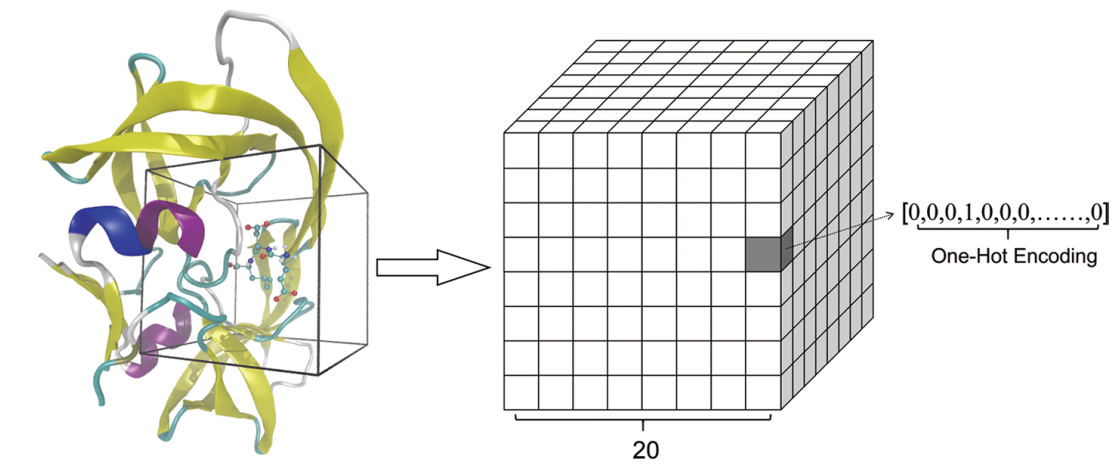
\includegraphics[width=0.5\textwidth]{images/one_hot.png}
    \caption{Featurization of the protein-ligand complexes. PDB ID 1a30 is shown as an example. In the default case, the resolution of $20\times20\times20$ and 28 categories of atomic types were used.}
    \label{fig:onehot}
\end{figure}

\section{Network}

The original paper presents 4 different network structures along with 3 ways of featurization. The network shown in the figure, combined with the featurization method above, achieved best performance on validation set.

\begin{figure}[!t]
    \centering
    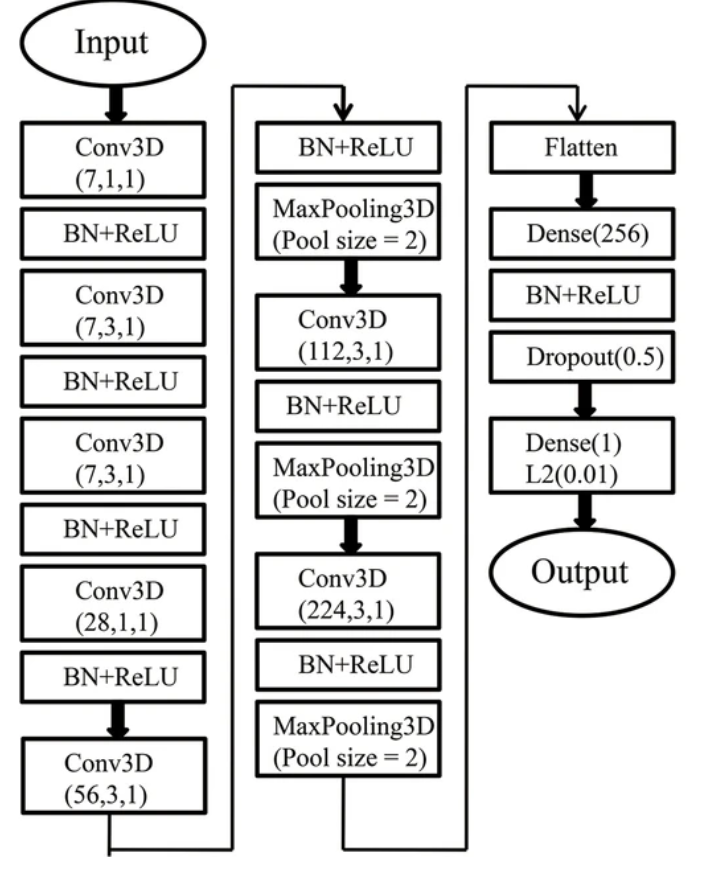
\includegraphics[width=0.35\textwidth]{images/CNN.png}
    \caption{Final CNN structure for Sfcnn network.}
    \label{fig:CNN}
\end{figure}

This network features 3D convolution layers with batch normalization and ReLU activation. L2 regularization was applied on the output layer to reduce the probability of overfitting and improve generalization.

\section{Reproduction}

\subsection{Dataset and Featurization}
The reproduction pipeline uses the same dataset and featurization method, resulting in a training 4D tensor shaped $(48520, 20, 20, 20, 28)$ and a testing 4D tensor shaped $(285, 20, 20, 20, 28)$.

\subsection{Data Storage}
It is worth noting that the original Sfcnn data storage uses the format of .pkl (pickle file), which concatenates the full arrays first, then dumps into the file at once. This approach requires to store and dispatch all the complexes' information within local memory, which would cause extremely high memory consumption due to the high training data volume and is unfeasible on normal computers.

Alternatively, our team switched to the format \texttt{.h5} (h5py file), which supports instant writing and solves the issue, resulting in a 40.1 GiB training grid.

\subsection{Network Structure}
The PyTorch network structure is similar to the original TensorFlow version except for two main differences:
\begin{enumerate}
    \item Due to the Conv3D API requirement in PyTorch, the input 4D tensor shape is permuted to (batch\_size, 28, 20, 20, 20).
    \item PyTorch lacks a direct L2 regularization API, so the final linear layer in the fully connected part is set with a weight decay to imitate the effect.
\end{enumerate}

\subsection{Training}
The training process is performed on training and validation sets. The validation set is partitioned from the training 4D tensor, indexed from 41000 to 48520, same as the original network. The final training set shape: $(41000, 20, 20, 20, 28)$, validation set shape: $(7520, 20, 20, 20, 28)$. The final dataset ratio is train : validation : test = 84.00\% : 15.42\% : 0.58\%.

Notice that the original training hyperparameters failed to converge in our experiments on the PyTorch network. Both the original hyperparameters and our current hyperparameter choice are presented in Table~\ref{tab:hyperparams}.

\begin{table}[!t]
\centering
\caption{Original/Reproduced hyperparameters}
\label{tab:hyperparams}
\begin{tabular}{lcc}
\toprule
Param & Original & Reproduced \\
\midrule
\textbf{lr (learning rate)} & 0.004 & 0.0015 \\
\textbf{batch size} & 64 & 32 \\
\textbf{dropout rate} & 0.5 & 0.15 \\
L2 regularization/FC weight decay & 0.01 & 0.01 \\
epochs & 200 & 200 \\
\bottomrule
\end{tabular}
\end{table}

\section{Results}

\subsection{Metrics}
The performance of Sfcnn is measured by the following four main metrics:

\begin{align*}
\mathrm{RMSE} &= \sqrt{\frac{1}{N} \sum_{i=1}^{N} (y_{\text{predict}} - y_{\text{true}})^2} \\
\mathrm{MAE} &= \frac{1}{N} \sum_{i=1}^{N} |y_{\text{predict}} - y_{\text{true}}| \\
\mathrm{SD} &= \sqrt{\frac{1}{N-1} \sum_{i=1}^{N} ((a y_{\text{predict}} + b) - y_{\text{true}})^2} \\
\mathrm{R} &= \frac{\mathbb{E}[(y_{\text{predict}} - \mu_{y_{\text{predict}}})(y_{\text{true}} - \mu_{y_{\text{true}}})]}{\sigma_{y_{\text{predict}}} \sigma_{y_{\text{true}}}}
\end{align*}

where $a$ and $b$ represent the slope and intercept of the linear regression line of the predicted and measured values. $\mathbb{E}[\cdot]$ denotes the expectation. $\mu_{y_{\text{predict}}}$ and $\mu_{y_{\text{true}}}$ are the means, and $\sigma_{y_{\text{predict}}}$ and $\sigma_{y_{\text{true}}}$ are the standard deviations of the predicted and true values, respectively.

\begin{table}[!t]
\centering
\caption{Performance Metrics Comparison on CASF-2016 Core Set}
\label{tab:metrics}
\begin{tabular}{lcc}
\toprule
Metrics & Reproduced Sfcnn & Original Sfcnn \\
\midrule
\textbf{Pearson R} & 0.7286 & 0.7928 \\
RMSE & 1.5481 & 1.3263 \\
MAE & 1.2579 & 1.0277 \\
SD & 1.4892 & 1.3252 \\
\bottomrule
\end{tabular}
\end{table}

Notice that despite the original Sfcnn presents better scores in all the metrics, its performance is doubtful since its reproduced training process did not reach convergence.

Due to the data storage mentioned above and the author's failure to respond to the request raised by another individual of providing the original (.pkl) training set on GitHub\footnote{\url{https://github.com/bioinfocqupt/Sfcnn/issues/1}}, \textbf{the original training process is irreproducible}.

The training curves are presented below as comparison.

\begin{figure}[!t]
    \centering
    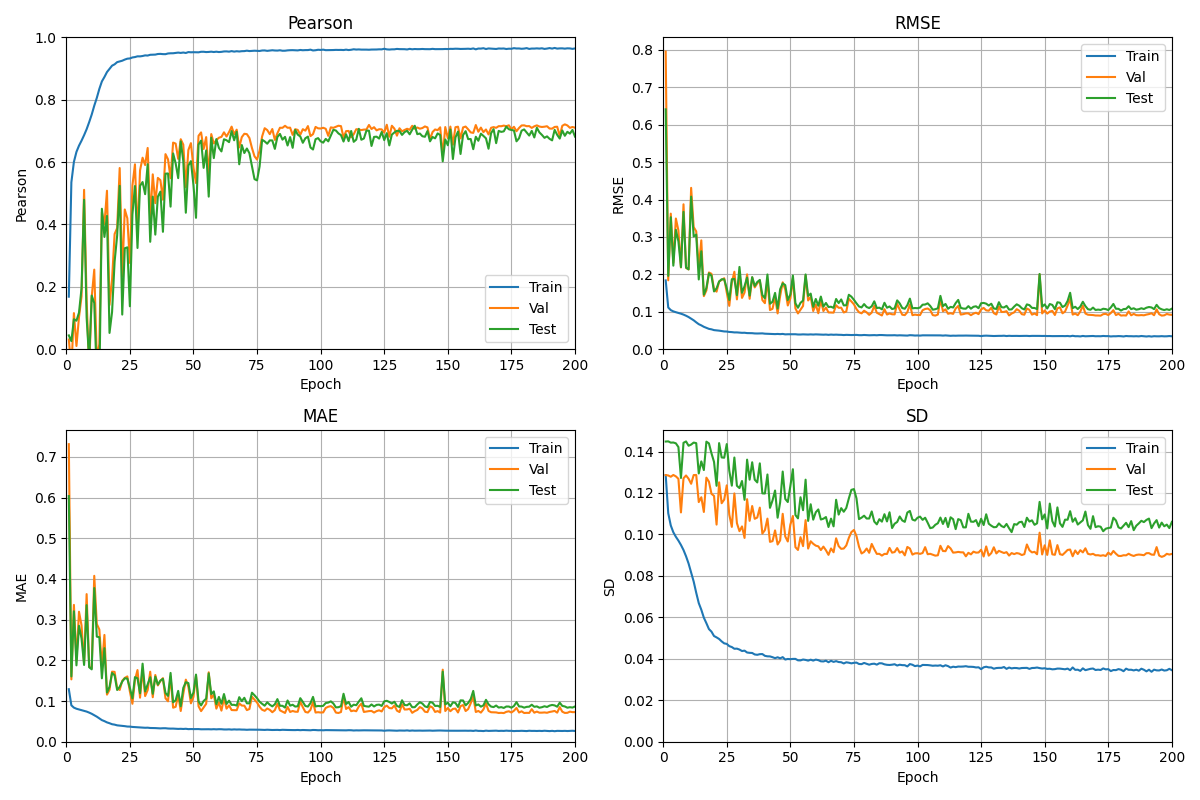
\includegraphics[width=0.5\textwidth]{images/normal_converge.png}
    \caption{Training process for Reproduced Parameters}
    \label{fig:ReproducedPlot}
\end{figure}

\begin{figure}[!t]
    \centering
    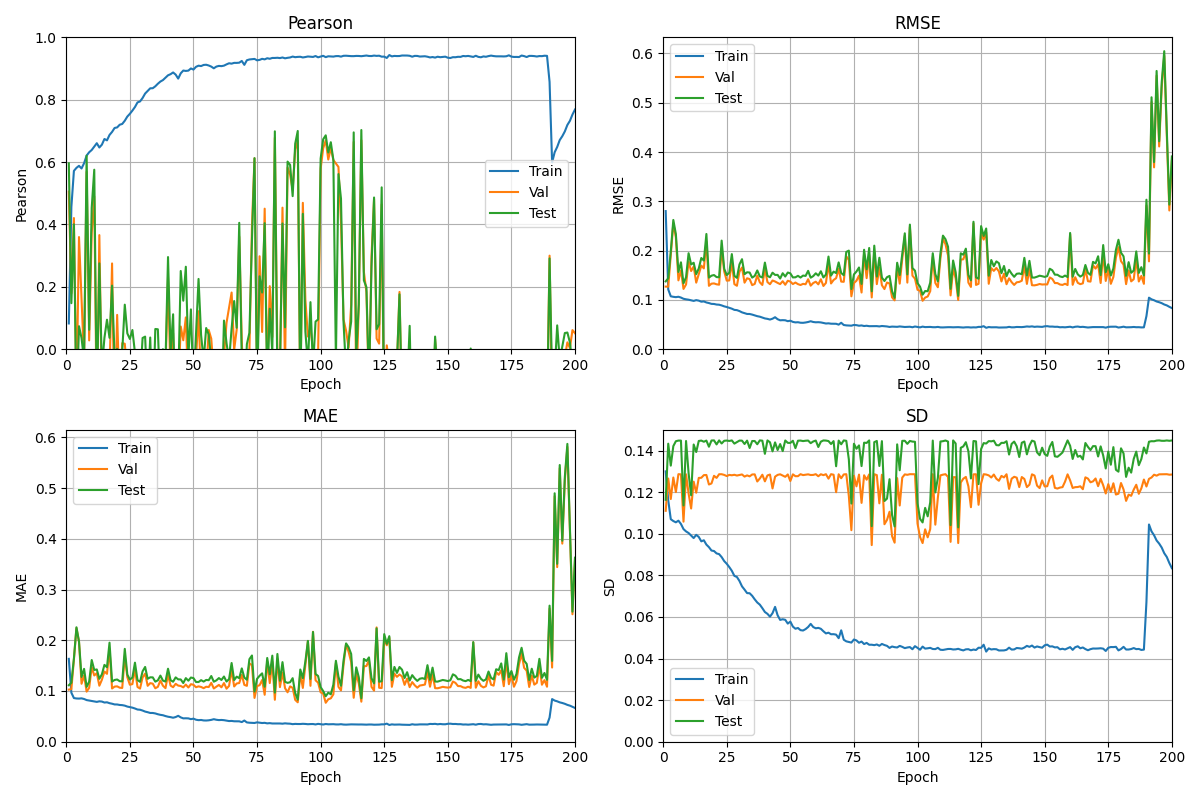
\includegraphics[width=0.5\textwidth]{images/origin_param.png}
    \caption{Training process for Original Parameters}
    \label{fig:OriginalPlot}
\end{figure}

After discussion, our team will take the \textbf{reproduced (convergent) result} as the normal performance of the Sfcnn network and will apply it to the next part of AlphaFold3 result assessing.

\section{AlphaFold3 Predictions}

\subsection{Dataset}
The assessment dataset used is the CASF-2016 core set mentioned above except for 6 specific proteins with overly complex structure for AlphaFold3 to make useful predictions, resulting in total \textbf{279} proteins.

Proteins with more than 5 Isomorphic/Heterogeneous Chains are deemed too complex and excluded. Those proteins are listed below:

\begin{table}[!t]
\centering
\caption{6 complex protein structures}
\label{tab:complex}
\begin{tabular}{lc}
\toprule
PDB ID & Isomorphic/Heterogeneous Chains \\
\midrule
2xb8 & 12 \\
2ymd & 10 \\
3n76 & 12 \\
3n7a & 12 \\
3n86 & 12 \\
4ciw & 12 \\
\bottomrule
\end{tabular}
\end{table}

\subsection{WorkFlow}

\paragraph{Online Server}
Each protein structure is generated manually on the \textit{Chai-1 online server}\footnote{\url{https://lab.chaidiscovery.com/dashboard}} instead of the AlphaFold3 online server\footnote{\url{https://alphafoldserver.com/}} because it doesn't allow specific ligand SMILES (Simplified Molecular Input Line Entry System) code. The MSA (Multiple Sequence Alignment) option is selected with algorithm \textit{MMseqs2} for each generation.

\paragraph{Docking}
Results generated on the server are downloaded as zip files, each containing multiple scoring ranks and detailed metrics. The structure file with the highest rank (\texttt{pred.rank\_0.cif}) is used as the model result for assessment.

To avoid potential issues in converting .cif files\footnote{Crystallographic Information File} to .pdb\footnote{Protein Data Bank} and .mol2\footnote{Tripos molecule structure format} files, the structure files are parsed using the \texttt{MMCIFParser} provided in the Python library Bio.PDB, then go through the featurization and grid mapping process directly.

Notice that in the results of AF3, certain atoms or isotopes are not included in the 14 pre-set atom types; those atoms are included in the \texttt{other} part of the pre-set types.

\paragraph{Scoring}
The testing grid for predicted structures is scored using the reproduced network, loaded with the pre-trained weight which shows the above performance (Pearson 0.728). Detailed analysis of the PLA result and metrics will be analyzed in the following section.

\section{External Library Usage}

\begin{itemize}
    \item \textbf{PyTorch}: Neural Networks used in agents are built by both of us from scratch.
    \item \textbf{Gymnasium}: The training environment is designed and built by both of us based on Gymnasium's vectorized environment from scratch.
    \item \textbf{Viztracer}: This tracing tool helps us to the performance bottleneck of the agents.
    \item \textbf{Pandas}: This library is used to store and analyze the training data.
    \item \textbf{Numpy}: This library is used to store and process the training data.
    \item \textbf{Matplotlib}: This library is used to plot the training loss curve.
\end{itemize}

\section{Conclusion}
Some Conclusions here.

\section{Competing interests}
No competing interest is declared.

\section{Author contributions statement}
G.Y., L.T., and J.C. conceived the experiment(s), conducted the experiment(s), analyzed the results, and wrote and reviewed the manuscript.

\section{Acknowledgments}
The authors thank the anonymous reviewers for their valuable suggestions. This work is supported in part by funds from the National Science Foundation (NSF: \# 1636933 and \# 1920920).

% \bibliographystyle{plain}
% \bibliography{reference}

\end{document}